\chapter{Requirements and Technological Context}

As discussed in in the introduction \ref{sec:scope}, the main aim is the development of a VS Code Language extension that operates on par with
well-established tooling for other programming languages. The following requirements define the expected capabilities and characteristics the extension must demonstrate.

\begin{multicols}{2}
  \subsection*{Functional Requirements}
  \begin{enumerate}
    \item The extension must provide syntax highlighting for the target language, differentiating keywords, operators, literals, and identifiers.
    \item The extension must provide basic code completion suggestions based on language keywords and the abstract syntax tree (AST) generated by Langium.
    \item The extension must be able to validate data types within the language, providing warnings or errors when type mismatches occur.
    \item The extension must perform semantic analyses to detect invalid constructs, undefined variables, and other semantic errors.
    \item The extension must display syntax and semantic error messages in the editor in real-time as the user edits the code.
    \item The extension must utilize the Langium framework for language specification, parser generation, and language service implementation.
  \end{enumerate}

  \columnbreak

  \subsection*{Non-Functional Requirements}
  \begin{enumerate}
    \item The extension must respond to user edits with syntax and semantic feedback within 100-250ms for files of average size.
    \item The extension must provide a user-friendly experience that is consistent with other popular VS Code extensions.
    \item The extension must be structured and commented in a way that allows future developers to understand and extend its functionality easily.
    \item The extension must be compatible with the latest version of Visual Studio Code at the time of its release and be developed using Langium, with consideration for future maintenance and version support.
    \item The extension must be able to handle files of immense size (around 10000 lines) of code within the bounds of 1 second.
    \item The extension must be delivered with clear and comprehensive documentation, including installation, usage, and extension of its features.
  \end{enumerate}
\end{multicols}

\section{Alternative Technologies}

This extension is implemented using \textbf{Langium}, which itself builds upon the standardized \textbf{Language Server Protocol (LSP)} \cite{LSP}, yet
there are several other technologies and approaches available for creating Visual Studio Code language extensions. At its core, the LSP allows tooling for programming
languages to be developed in a modular, editor-independent manner, making it possible to implement a language server in any language that can communicate via JSON-RPC.

One common approach is to implement a language server using general-purpose programming languages (e.g., TypeScript, Java, or Rust) combined with parser generation libraries.
Technologies such as \textbf{Jison}~\cite{Jison}, \textbf{Nearley}~\cite{Nearley}, and \textbf{PEG.js}~\cite{PEGjs} offer a range of options for specifying a language's grammar
and creating a parser. These libraries vary in design and capabilities and may need extra components, such as dedicated lexers and scoping to enable fully-fletched tooling.

In contrast, more comprehensive technologies such as \textbf{ANTLR}~\cite{ANTLR} and \textbf{Langium} go beyond
basic parsing. ANTLR provides a mature and highly optimized lexer and parser generation framework that is widely used across many programming languages, while Langium offers
an end-to-end solution for language engineering - including built-in support for scoping, indexing, and validation - making it especially suited for creating fully
featured language servers.

For basic syntax highlighting and lexical analysis, \textbf{TextMate}-style grammars~\cite{TextMate} can be used, offering a lightweight approach when deep semantic understanding is not required.
Meanwhile, incremental parsing frameworks such as \textbf{Tree-sitter}~\cite{Treesitter} have gained popularity for their ability to provide high-performance syntax parsing and error recovery,
making them ideal for tooling that operates on very large files.

\chapter{Langium}

Langium is a young language engineering framework inspired by the accomplishments of \verb|Xtext|, striving to evolve into a similarly comprehensive and widely-used technology stack.\cite{LangiumWeb}
Its goal is to lower the barrier to entry for language design and implementation, opening the field to new users and fostering the growth of its user base.
To achieve this, Langium embraces the extensibility of the Visual Studio Code ecosystem and its extension pipeline, provides a rich set of built-in
capabilities while strongly focusing on quality and maintainability, ensuring that newcomers and experienced developers alike can build robust, sustainable language tooling.

Although Langium is capable of defining general-purpose languages, its design is primarily optimized for domain-specific languages (DSLs), targeting languages with a limited range of abstraction and complexity.
Creating a fully featured GPL is a highly exhaustive endeavor that demands extensive semantic modeling, thorough tooling, and a substantial team of developers.
In contrast, Langium is tailored to lower the entry barrier for language design, making it an ideal choice for building DSLs that solve specific, well-defined problems.
\\

\section*{Technical Details \& Features}

Langium is an open-source framework for building programming languages and DSL tooling, distributed under the MIT license and backed by the Eclipse Foundation \cite{LangiumGit}.
Its open-source nature encourages collaboration and continuous improvement through active engagement with the community.
\begin{multicols}{2}
  \begin{itemize}
    \item At its core, Langium builds upon \verb|Chevrotain|, a customizable JavaScript parser engine that is highly optimized. Chevrotain constructs an internal prediction DFA \cite{sujew2022enabling}
          from the grammar's production rules to implement its configurable LL($k$) lookahead mechanism, allowing the look-ahead depth $k$ to be tuned for both performance and
          expressiveness. Moreover, Langium exposes this configurability directly - authors can adjust the parser's \verb|maxLookahead| setting to manage grammar complexity and
          parsing speed. After parsing, Chevrotain produces a Concrete Syntax Tree (CST), which Langium then converts into a typed Abstract Syntax Tree (AST) using the visitor pattern:
          by extending Chevrotain's own Visitor interface, Langium traverses the CST and emits AST nodes, preserving semantic structure while discarding syntactic noise.
          Langium does not incrementally parse documents (i.e., it does not reuse prior parse results to update only modified regions), yet it still offers significant performance
          benefits compared to alternative engines \cite{Chevrotain}, complementing its generation of precise ASTs and CSTs and its robust error recovery capabilities. The error recovery is
          implemented with single-token insertion and deletion strategies to correct unexpected or missing tokens, alongside rule-level resynchronization that discards input until a defined
          recovery point is reached, to maintain parser continuity in the face of syntax errors.
    \item Langium provides a custom DSL using the \code{.langium} extension to define the grammar on which everything else is built upon. This DSL closely resembles an EBNF grammar,
          augmenting basic BNF with regex-like operators, language constructs for assignments and typing, and built-in cross-referencing. Cross-referencing enables production rules to declare relations to one another, which are resolved during a document's linking phase.
          Once defined, the core grammar is converted into a Chevrotain compatible JSON view, which when consumed by the parser, produces a fully typed AST. While linking, the AST is traversed and any
          cross-references resolved by checking the reference against the computed scope of each possible reference holder.
    \item In addition to its core language capabilities, Langium offers further extensibility: its generator API traverses ASTs and CSTs to produce arbitrary outputs
          - whether transpiled or compiled code, structured data formats such as JSON, XML, or Markdown, or custom domain-specific representations - and thus supports downstream
          processing, tooling, or integration into build and deployment pipelines.
          Langium projects can also be scaffolded into a command-line interface, registering commands for parsing, validation, generation, and LSP serving; each command invokes the
          corresponding language services to parse source files, apply validation rules, execute generator or interpreter routines, and emit results, thereby enabling a cohesive
          suite of tools, that leverage Langium's core capabilities across diverse environments.
    \item Leveraging established and widely adopted ecosystems is central to the design of Langium, allowing it to benefit from mature tools, protocols, and conventions.
          As a result, it adopts the LSP - standardizing language tooling across platforms and environments - to enable seamless integration with editors and IDEs such as Visual Studio Code and Eclipse Theia.
          In the same vein, it is developed in TypeScript and distributed via npm, which allows it to build upon the robust tooling, typing support, and package infrastructure of the JavaScript and TypeScript landscapes.
    \item To further streamline the DSL development process, Langium provides a dedicated scaffolding tool based on \verb|Yeoman|. This generator automates the creation of a
          fully configured project, including a grammar template, build pipelines, and example code for parsers, validations, and editors. Removing boilerplate setup provides a
          standardized structure to build upon and saves developers significant time and effort, making Langium a practical and accessible platform.
  \end{itemize}
\end{multicols}

\section{High-Level Architecture Diagram}
update diagram such that cusomt services also extends the lsp providers
\begin{figure}
  \centering
  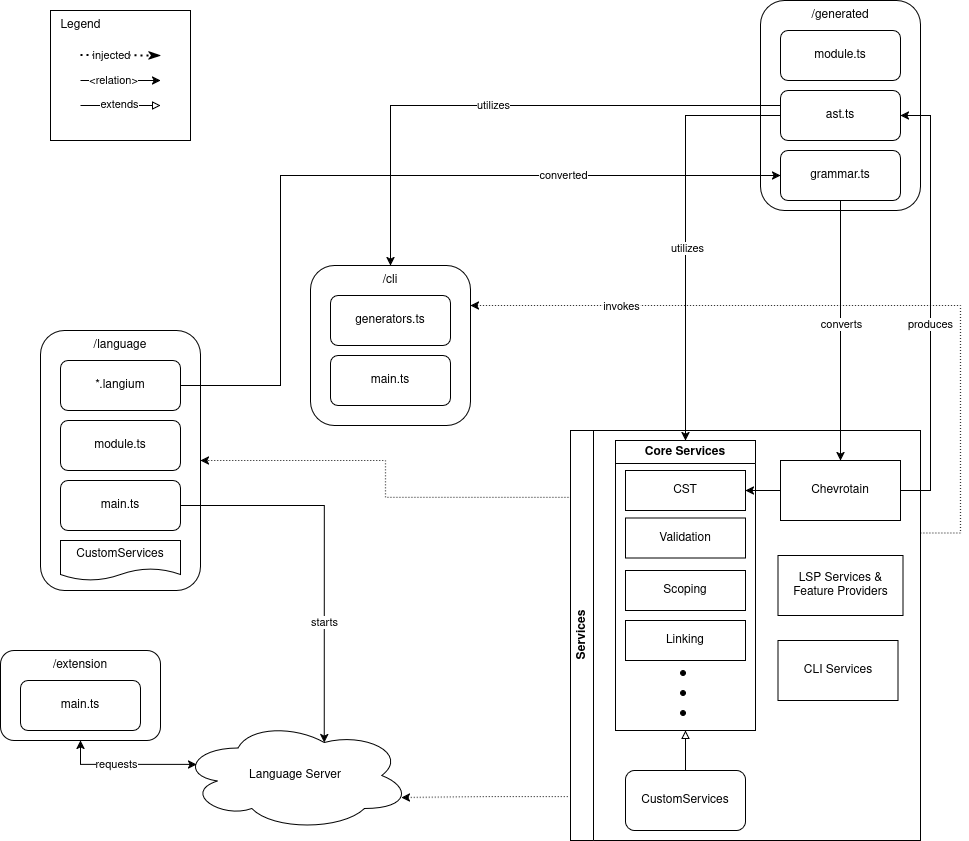
\includegraphics[width=\textwidth]{graphics/langiumArchitecture.png}
  \caption{Architecture overview of a Langium project}
  \label{fig:langium-architecture}
\end{figure}


\section{Module Decomposition}

Langium projects can easily be created with the support of the scaffolding tool \verb|Yeoman|, producing a structured mock project including a sample language definition.
Most of the definitions are found in the \verb|src| directory \ref{fig:langium-architecture}, encompassing functionality for the Language Server, the extension and actual language tooling.

\begin{description}
  \item[\code{language/}] Assembles the core of any Langium project. It includes the \code{.langium} file, in which the custom language grammar is defined, as well as
    the code that starts the Language Server with all necessary services bundled.
  \item[\code{cli/}] Provides functionality for CLI interactions, command parsing, and generators. The generators in this folder invoke processes that generate artifacts
    from the language and input files; they are typically used only offline and are called once rather than continuously via the CLI and support efficient pipelining.
  \item[\code{extension/}] Contains the VS Code extension bootstrap code needed to connect to the Language Server and utilize LSP support features.
    All mentioned folders except the one containing CLI logic are bundled into the extension itself.
  \item[\code{generated/}] Contains artifacts produced from the grammar definition in the \code{.langium} file. This includes TypeScript AST type definitions,
    which are essential for further analysis and validation, as well as the preliminary parsed grammar rules formatted for the Chevrotain engine to generate parsers.
  \item[\textsf{Services}] The Services in Langium are a collection of utility classes and helper functions offered to every component of a language project via
    dependency injection. They cover an extensive range of functionality, from LSP-specific features - such as providers for context-aware code completion, rich hover
    tooltips, signature help, go-to-definition and find-references - to core language utilities that expose parsed documents as both AST and CST models, manage workspace
    state and context information (including indexing, scoping, and name resolution), synchronize the in-memory document model and perform validation checks.
    Because the parts are wired up as an injectable service, precise consumptions of the capabilities needed is possible. Moreover, Langium enables developers to swap in
    custom implementations of services by extending the corresponding default classes, and these services have to be wired into the DI container manually \ref{sec}.
    By default, the validation logic is located in the \code{language/} directory; subsequently, I placed additional custom services there.
    However, as these services grow in both number and complexity, it may be more appropriate to organize them in a dedicated module or folder.
\end{description}

Both \code{module} files share analogous responsibilities by encapsulating dependency-injection setup and service registration for the language environment.
The generated module is produced automatically from the grammar definition and offers two DI fragments, one that registers shared-core services such as AST
reflection and another that configures the parser, the Chevrotain grammar factory and language metadata. In contrast the main module is handwritten and imports
Langium's default core and shared fragments, registers any custom services such as validators, scope providers and caches, invokes \code{inject} to assemble the full
service container and exposes a \code{createServices} factory.

Although the core logic resides in \code{/src}, other files of interest reside at the project root including configurations for npm/node and Langium itself:
\code{language-configuration.json}, which governs editor behaviors such as comment delimiters, bracket pairs and auto-closing rules, and
\code{langium-config.json}, which declares settings like the language ID, grammar entry point, target file extensions and maximum lookahead.
In particular, the \code{syntaxes} config property enables the generation of either a `.monarch.ts` (for Monaco-based editors) and a `.tmLanguage.json` file (for TextMate-based engines).
The TextMate grammar maps regex patterns to semantic scopes that underpin VS Code's coloring, bracket
matching and code folding, and is the one consumed by the extension. Customizing the syntax files allows developers to implement nuanced highlighting
- such as semantic theming and advanced pattern recognition - that cannot be exhaustively defined by grammar rules alone \cite{EDKarlsson2022Discussion604}.

Notably, projects initialized with the scaffolding tool include extra files not discussed; these include, amongst others, the Monarch grammar files, Vite-related configs,
and setup scripts - scaffolded for a web demo but can be removed when solely focusing on developing the language tooling extension.

\section{Language Server Protocol}
control flow of lsp from file to lsp to editor

custom providers, computators

\section{Data Flow and Control Flow}


\chapter{Implementation Details}
\label{sec:langium-grammar}
\section{Langium Grammar Definition for \textit{MiniProb}}

A Langium grammar definition primarily consists of rules: \code{<Rulename>: <production_result>} and terminals: \code{terminal <name>: <result>} defining the language
in accordance of conventional grammatical specifications. In addition, it must also include keywords specifying the grammar name also used in the AST: \code{grammar <name>},
and to determine the start from which a document should be parsed: \code{entry <RootRulename>: <production_result>}.
In this case, the production result describes the whole parsable document and therefore acts as the root node of the AST.
\\
Also mention the LL (2) parsability and which tokens demand a 2 lookahead ()
The code excerpts in the following sections are all taken from the original MiniProb Langium grammar (\ref{list:langium-grammar}) and, for easier digestion,
have been truncated; each snippet focuses respectively on the core rules, the expression system, and the terminal and type definitions.
\subsection*{Core rules}

The code excerpt shown here defines 'MiniProb' as the grammar name and sets the \code{Program} rule as the entry point, adhering to nominal abstraction by
referring to each MiniProb-parsed document as a program. Lines of interest include line 8 - showing that every MiniProb program consists of some global declarations
followed by at least on function - and line 4, which allows for file import of other MiniProb programs at the beginning of the document.

The \code{FileImport} rule emulates the C preprocessor's "\#include" directive by requiring a literal match of the \texttt{\#include} keyword followed by a
file name token (terminal \code{STRING}). Generally during parsing, each line is evaluated either against these fixed string keywords or against any matching terminals (order of match).
As the file names have to be retrievable once it is time to compute the scope \ref{sec:customservices}, they are made accessible through the AST
, with each FileImport-node containing a \texttt{file} property that stores the corresponding value.

This declaring of \textit{assignments} (here also referred to as fields) is a central feature of the Langium DSL, which binds other grammar rules or literal strings for subsequent retrieval and use in AST-based computations.
Because all production rules extend upon the \code{AstNode} base class, the assigned fields share a common origin allowing polymorphic access and seamless traversal and processing of every rule-node;
the exception being string literals, which are treated as language specific keywords (eg. "while", "throw"). Fields can either be single valued (line 24) or multi-valued (line 12)
in which case an array of the referred rule is created instead of a single instance.
Furthermore, fields may be assigned optional rules, which are backed in the AST by nullable values (lines 5, 6, 16), or if multi-valued,
by types that default to \underline{undefined} (lines 4, 8). It is also possible to directly mark assignments as optional (line 20), if so,
the AST denotes the property as a boolean flag indicating whether the field was present.

Bracketed annotations (\code{[<Rule>:<Value>]}, line 16) impose stronger cross-referential constraints by requiring
that the target symbols be defined elsewhere in the document/scope and hold a field with the same value; such cross-references are resolved during the scoping phase (see Figure \ref{fig:controlflow}).
When a field references multiple distinct rules, the \code{type} keyword has to be used (line 2) unifying the rules into a single symbol, which generates an union type within the AST \cite{typescript-unions-intersections}.
In particular, all union members must share the same underlying value type: consider line 16, 12 and 20, Lval refers to either Param or Decl expecting the resolution to occur
over an ID.

\begin{minted}[linenos, breaklines]{yaml}
grammar MiniProb
type DeclOrParam = Decl | Param;
entry Program:
    (fileImports+=FileImport)*
    probabilisticQuery=PROB_QUERY? // not tested: out of scope
    formula=FORMULA? // not tested: out of scope
    'program:'?
    (declarations+=Decl ';')* functions+=Func+;
FileImport:
    '#include' file=STRING;
Decl:
    type=Type names+=ID (',' names+=ID)*;
.
.
Lval:
    ref=[DeclOrParam:ID] ('['index=Expression']')?;
.
.
Param:
    type=Type byRef?='&'? name=ID;
ArgList:
    arguments+=Arg (',' arguments+=Arg)*;
Arg:
    expression=Expression; //only expression and no by-ref symbol (could be replaced)
.
.
\end{minted}

\subsection*{Expressions}

Most of the expression system is omitted here, as it closely follows the \textit{operator-precedence grammar} pattern common to LL parsers \cite{operatorPrecedence}.
Typically, a grammar defines a series of nonterminals - each corresponding to a distinct operator-precedence level (from primaries up to full expressions) - and structures its productions so as to eliminate left recursion while preserving left-associative evaluation at every level.
This arrangement guarantees that the parser can always choose the correct production with a single lookahead token, ensuring LL(1) compliance.

\begin{wrapfigure}{r}{0.40\textwidth}
  \centering
  \begin{forest}
    for tree={
    grow=south,
    edge={-stealth},
    l sep=0.2em,
    align=right,
    }
    [Expression
    [ProbabilisticAssignment?
    [LogicalOr\,(\texttt{||})
    [LogicalAnd\,(\texttt{\&\&})
        [Comparison\,(\texttt{< <= > >= == !=})
            [Term\,(\texttt{+ -})
                [Factor\,(\texttt{*})
                    [Division\,(\texttt{/ \%})
                        [Unary\,(\texttt{!})
                            [Primary]
                          ]
                      ]
                  ]
              ]
          ]
      ]
    ]
    ]
    ]
  \end{forest}
  \caption{Operator‐precedence hierarchy}
  \label{fig:op-prec-tree}
\end{wrapfigure}

In Langium, rules can be made to share other base classes than \code{AstNode} by utilizing the \code{infers} keyword. This is especially useful for creating a layered expression system, as all the levels infer from the top-most expression (line 3), which follows logical abstraction and enables dynamic and easy resolution of parsed expressions.
The lines depicted here have been selected because they include the \code{Probabilistic Assignment}, a construct particular to MiniProb (see \ref{sec:miniprob}), alongside the \code{Primary} rule, which defines the core forms to which all expressions ultimately resolve.
The topmost level of the precedence hierarchy was originally occupied by the disjunction operator (\code{||}), but was ultimately edged out by the probabilistic assignment. This behavior is enabled by another Langium specific command \code{infers}, which instructs a rule to create a new AST node based on the structure of the input.
In this case, an \code{Expression} is by default parsed as a \code{LogicalOr}, but immediately becomes a \code{Probabilistic Assignment} node as soon as the first curly brace is recognized (lines 2, 4). The remainder of the operator precedence follows conventional conventions, with the exception that '\code{*}' binds more loosely than division and modulo (see Figure~\ref{fig:op-prec-tree}).

All expression consist of \code{Primary}'s on an elementary level and can be either boolean, an integer literal, or a variable reference (\code{Lval}); treating \code{Lval} as a \code{Primary} makes variable accesses first-class expressions,
as is conventional in many languages. In addition, the production allows any expression to be wrapped in arbitrarily many parentheses which only delegate the inner expression without altering the meaning.

\begin{minted}[linenos, breaklines]{yaml}
ProbChoice:
    '{'numerator=Expression ':' denominator=Expression '}';
Expression:
    LogicalOr ({infer ProbabilisticAssignment.head=current} (probabilities+=(ProbChoice) fallbacks+=LogicalOr)+)?;
LogicalOr infers Expression:
.
.
.
Primary infers Expression:
    {infer BoolLiteral} literal=BOOL | 
    {infer IntLiteral} literal=IntegerLiteral |
    Lval |
    '(' Expression ')';
\end{minted}

\subsection*{Types and terminals}

The excerpt displayed here, defines the types alongside its literal lexical vocabulary. The nonterminal \code{Type} accepts either the literal keyword \code{bool} or an \code{IntType}. An \code{IntType} specifies if it's signed and of what width and may be converted to an \code{IntArray} if brackets are present (line 4).
The \code{IntegerLiteral} rule recognizes numeric constants with an optional printable sign. Together, these productions ensure that boolean types, integers, and arrays are adequately represented according to the \code{MiniProb} definition (\ref{sec:miniprob}).

Lexical terminals and hidden terminals are distinguished to control which tokens contribute to the final model. Terminals defined in lines 8-13 produce concrete tokens that appear in the parse tree as syntactic elements or attribute values; several of these declarations include a \code{returns} clause (lines 9, 12, 13) to instruct the parser on the semantic type to assign in
in the resulting node. Hidden terminals defined in lines 14-16 are recognized by the lexer but discarded before parsing, preventing formatting and commentary from influencing the structural representation.

Moreover, the \code{ID} terminal employs a \textit{negative lookahead} to exclude specific sequences from being recognized as identifiers (line 11). This mechanism ensures that boolean literals and integer prefixes are not misclassified as identifiers, preserving the distinct classification of reserved words and type prefixes without requiring further enforcements.

Finally, should input match multiple terminal patterns, the lexer resolves ambiguities by first selecting the pattern that consumes the most characters (longest-match rule) and then, in the event of equal length, the rule declared earlier in the grammar.

\begin{minted}[linenos, breaklines]{yaml}
Type:
    'bool' | IntType;
IntType:
    prefix=INT_PREFIX ({infer IntArray} '[' size=INT ']')?;
IntegerLiteral:
    sign=('+' | '-')? value=INT suffix=INT_PREFIX;

terminal INT_PREFIX: /[su][1-9][0-9]{0,8}/;
terminal BOOL returns boolean: /(true|false)/;
.
terminal ID: /(?!(true|false)|[su][1-9][0-9]*)[a-zA-Z_][a-zA-Z0-9_\.\:\~]*/;
terminal STRING returns string: /"(\\.|[^"\\])*"|'(\\.|[^'\\])*'/;
terminal INT returns number: /[0-9]+/;
hidden terminal WS: /\s+/;
hidden terminal ML_COMMENT: /\/\*[\s\S]*?\*\//;
hidden terminal SL_COMMENT: /\/\/[^\n\r]*/;
\end{minted}

\section{Type System and Semantic Checks}

Langium offers the option of formalizing semantic checks and type systems through a static validation service which can be registered in its dependency-injection framework.
Once registered, this service traverses the abstract syntax tree via a visitor pattern, invoking node-type specific validation routines at each step.
The following sections describe the implementation of static semantics and the design of the type system.

\subsection*{Validator}

The excerpt below presents the registration function exported from \code{validator.ts} that consolidates all validation routines for statically
verifying the parsed syntax tree. This function integrates those checks into the overall services infrastructure and is subsequently invoked in \code{module.ts} to
initialize the complete set of services. As noted, every AST node is processed during the validation phase. Each rule may declare one or more validation methods
(provided as an array). These methods receive two parameters - the node instance itself and a ValidationAcceptor - which is used to produce diagnostics shown in the editor, such as error markers, warnings, and informational messages.



\begin{minted}[linenos]{ts}
  export function registerValidationChecks(services: MiniProbServices) {
  const registry = services.validation.ValidationRegistry;
  const validator = services.validation.MiniProbValidator;
  const checks: ValidationChecks<MiniProbAstType> = {
    Lval: validator.checkArrayAccess,
    FuncCall: validator.checkFunctionCalls,
    Func: validator.checkFunctionDefinitions,
    .
    .
    .
    IntegerLiteral: validator.checkIntegerLiteral,
    Program: validator.checkMainOccurrences
  };
  registry.register(checks, validator);
}
\end{minted}

These validations are AST-driven logical procedures that verify specified conditions on the syntax tree. This means that validation is performed by statically inspecting
each node's structure, attributes, and inter-node relationships, without relying on runtime information or any other states.
Each procedure either invokes the \code{ValidationAcceptor} to report deviations when constraints are violated or lets the node pass unremarked when it
satisfies the criteria. As an example, consider the following \code{checkMainOccurrences} method, which enforces the invariant that a \code{main()} function must be defined exactly once in each program.
\begin{minted}[linenos]{ts}
  checkMainOccurrences(node: Program, accept: ValidationAcceptor) {
     const functionNames = node.functions.filter(f => f.name === "main")
            .map((f) => f.name);
     if (functionNames.length <= 0) {
      accept("error", 'Each program needs a \'main()\' function.', {
        node,
        property: "functions"
      });
     }
     .
     .
}
\end{minted}

Beyond basic AST-based checks, the analysis can be extended by incorporating models that augment node-level information with additional contextual or semantic data.
In these frameworks, the AST serves as the foundational seed from which richer representations and semantics are derived and maintained in dedicated structures.
This also enables the implementation of a custom type system whose validation routines are registered alongside other checks, allowing the validator to
invoke type-checking services during the validation phase.

The type system used here is much simpler than those found in mainstream GPLs and comprises just four files. The \code{operation.ts} and \code{compatible.ts}
modules each contain targeted logic: for assignments and function calls, \code{compatible.ts} verifies that the involved types are compatible (the integer corner cases are handled here as well),
while for all expressions and operators, \code{operation.ts} checks that the operand types are valid for the given operation. Both return their judgement as a simple boolean to
the validator, which can react accordingly - and already aware of the involved types - produce detailed error messages.

The \code{description.ts} module defines the core vocabulary of the type system, including a TypeDescription union (e.g. \code{BooleanTypeDescription}, \code{IntegerTypeDescription}, etc.),
factory functions (\code{createIntegerType}, \code{createErrorType}, …) and predicates (\code{isIntegerType}, \code{typeToString}, …). It also introduces an explicit
\code{ErrorTypeDescription} to represent and propagate type-checking failures without interrupting the overall inference process. The \code{infer.ts} file leverages these
descriptions by traversing the AST: for each node it recursively infers subexpression types - adhering to the system's inference compatibility rules (see axiomatic rules below)-
and returns either a concrete \code{TypeDescription} or the \code{ErrorTypeDescription} when mismatches occur, with a simple cache mechanism preventing infinite recursion and boosting performance.

The cache is instantiated anew for each inference run on a node, eliminating any risk of residual data or cross-contamination and ensuring fully deterministic results.
However, because it isn't persisted between runs, identical subtrees get re-evaluated on every pass, which can introduce redundant work.
Unlike incremental parsing systems that retain state to avoid reprocessing unchanged regions, this approach performs a complete, conventional traversal each time.

As an example ....
\begin{minted}{ts}
  checkUnaryExpressions(node: LogicalNegation, accept: ValidationAcceptor) {
    const map = this.getTypeCache();
    const operandType = inferType(node.operand, map);

    if (isErrorType(operandType)) {
      accept('error', operandType.message, { node: operandType.source ?? node });
      return;
    }
    if (!isLegalOperation(node.operator, operandType)) {
      accept(
        'error',
        `The operation '${node.operator}' is not possible on type '${typeToString(operandType)}'`,
        { node, property: 'operand' }
      );
    }
  }
\end{minted}

\subsubsection*{Base axioms}
\[
  \begin{array}{rcll}
    \tau   & ::=                                & \mathsf{Bool}
    \;\bigm|\; \mathsf{Int}_{s,w}
    \;\bigm|\; \mathsf{Array}\langle\mathsf{Int}_{s,w}\rangle
           & (s\in\{\top,\bot\},\;0<w<2^{29}-1)                 \\[1ex]
    \Gamma & ::=                                & \emptyset
    \;\bigm|\; \Gamma,\,x:\tau
  \end{array}
\]
\[
  \frac{}{\Gamma \vdash \mathit{true} : \mathsf{Bool}}
  \; (\textsc{T-True}), \quad
  \frac{}{\Gamma \vdash \mathit{false} : \mathsf{Bool}}
  \; (\textsc{T-False})
\]
\[
  \frac{}
  {\Gamma \;\vdash\; n^{(s,w)} : \mathsf{Int}_{s,w}}
  \; (\textsc{T-IntLit}), \quad
  where\;
  s \in \{\top, \bot\},
  \quad
  w \in \mathbb{N},
  \quad
  1 \;\le\; w \;\le\; 2^{29}-1
\]
\[
  \frac{\vdash\;\mathsf{Int}_{s,w}\;}
  {\vdash\;\mathsf{Array}\langle\mathsf{Int}_{s,w}\rangle}
  \quad(\textsc{Ty-Array})
\]

\subsubsection*{Inference rules}
\begin{multicols}{2}

  \[
    \begin{aligned}
      \frac{x:\tau\in\Gamma}{\Gamma \vdash x : \tau}
       & (\textsc{T-Var})   \\[2ex]
      \frac{\Gamma \vdash e : \tau}{\Gamma \vdash (\,e\,) : \tau}
       & (\textsc{T-Paren}) \\[2ex]
      \frac{\Gamma \vdash e : \mathsf{Bool}}
      {\Gamma \vdash \neg e : \mathsf{Bool}}
       & (\textsc{T-Not})
    \end{aligned}
  \]

  \[
    \begin{aligned}
      \frac{\Gamma \vdash e_1 : \mathsf{Int}_{s_1,w_1}
      \quad
      \Gamma \vdash e_2 : \mathsf{Int}_{s_2,w_2}}
      {\Gamma \vdash e_1 * e_2 : \mathsf{Int}_{s_{\,s_1\lor s_2},\,\max(w_1, w_2)}}
       & (\textsc{T-Mult}) \\[1ex]
      \frac{\Gamma \vdash e_1 : \mathsf{Int}_{s_1,w_1}
      \quad
      \Gamma \vdash e_2 : \mathsf{Int}_{s_2,w_2}}
      {\Gamma \vdash e_1 / e_2 : \mathsf{Int}_{s_{\,s_1\lor s_2},\,\max(w_1, w_2)}}
       & (\textsc{T-Div})  \\[1ex]
      \frac{\Gamma \vdash e_1 : \mathsf{Int}_{s_1,w_1}
      \quad
      \Gamma \vdash e_2 : \mathsf{Int}_{s_2,w_2}}
      {\Gamma \vdash e_1 \bmod e_2 : \mathsf{Int}_{s_{\,s_1\lor s_2},\,\min(w_1, w_2)}}
       & (\textsc{T-Mod})  \\[2ex]
      \frac{\Gamma \vdash e_1 : \mathsf{Int}_{s_1,w_1}
      \quad
      \Gamma \vdash e_2 : \mathsf{Int}_{s_2,w_2}}
      {\Gamma \vdash e_1 + e_2 : \mathsf{Int}_{s_{\,s_1\lor s_2},\,\max(w_1, w_2)}}
       & (\textsc{T-Add})  \\[1ex]
      \frac{\Gamma \vdash e_1 : \mathsf{Int}_{s_1,w_1}
      \quad
      \Gamma \vdash e_2 : \mathsf{Int}_{s_2,w_2}}
      {\Gamma \vdash e_1 - e_2 : \mathsf{Int}_{s_{\,s_1\lor s_2},\,\max(w_1, w_2)}}
       & (\textsc{T-Sub})
    \end{aligned}
  \]

  \[
    \begin{aligned}
      \frac{\Gamma \vdash e_1 : \mathsf{Int}_{s,w}
        \quad
        \Gamma \vdash e_2 : \mathsf{Int}_{s,w}}
      {\Gamma \vdash e_1 < e_2   : \mathsf{Bool}}
       & (\textsc{T-Lt})  \\[1ex]
      \frac{\Gamma \vdash e_1 : \mathsf{Int}_{s,w}
        \quad
        \Gamma \vdash e_2 : \mathsf{Int}_{s,w}}
      {\Gamma \vdash e_1 <= e_2 : \mathsf{Bool}}
       & (\textsc{T-Le})  \\[1ex]
      \frac{\Gamma \vdash e_1 : \mathsf{Int}_{s,w}
        \quad
        \Gamma \vdash e_2 : \mathsf{Int}_{s,w}}
      {\Gamma \vdash e_1 > e_2   : \mathsf{Bool}}
       & (\textsc{T-Gt})  \\[1ex]
      \frac{\Gamma \vdash e_1 : \mathsf{Int}_{s,w}
        \quad
        \Gamma \vdash e_2 : \mathsf{Int}_{s,w}}
      {\Gamma \vdash e_1 >= e_2 : \mathsf{Bool}}
       & (\textsc{T-Ge})  \\[2ex]
      \frac{\Gamma \vdash e_1 : \tau
        \quad
        \Gamma \vdash e_2 : \tau}
      {\Gamma \vdash e_1 == e_2 : \mathsf{Bool}}
       & (\textsc{T-Eq})  \\[1ex]
      \frac{\Gamma \vdash e_1 : \tau
        \quad
        \Gamma \vdash e_2 : \tau}
      {\Gamma \vdash e_1 \:!= e_2 : \mathsf{Bool}}
       & (\textsc{T-Neq}) \\[2ex]
      \frac{\Gamma \vdash e_1 : \mathsf{Bool}
        \quad
        \Gamma \vdash e_2 : \mathsf{Bool}}
      {\Gamma \vdash e_1 \:\&\&\: e_2 : \mathsf{Bool}}
       & (\textsc{T-And}) \\[1ex]
      \frac{\Gamma \vdash e_1 : \mathsf{Bool}
        \quad
        \Gamma \vdash e_2 : \mathsf{Bool}}
      {\Gamma \vdash e_1 \:||\: e_2 : \mathsf{Bool}}
       & (\textsc{T-Or})
    \end{aligned}
  \]
\end{multicols}

\[
  \frac{
    \Gamma \vdash e_1 : \tau
    \quad
    \Gamma \vdash e_2 : \mathsf{Int}_{s,w}
    \quad
    \Gamma \vdash e_3 : \mathsf{Int}_{s,w}
    \quad
    \Gamma \vdash e_4 : \tau
  }
  {\Gamma \vdash e_1 \{\,e_2 :\!:\! e_3\}\, e_4 : \tau}
  \quad(\textsc{T-ProbAssign})
\]

\[
  \begin{aligned}
    \frac{\Gamma\vdash e : \mathsf{Array}\langle\mathsf{Int}_{s,w}\rangle
      \quad
      \Gamma\vdash i : \mathsf{Int}_{s,w}}
    {\Gamma\vdash e[i] : \mathsf{Int}_{s,w}}
     & (\textsc{T-Index})     \\[2ex]
    \frac{\Gamma \vdash e_1 : \mathsf{Int}_{s_1,w_1}
      \quad
      \Gamma \vdash e_2 : \mathsf{Int}_{s_2,w_2}}
    {\Gamma \vdash \mathrm{Bernoulli}(e_1,e_2) : \mathsf{Int}_{\bot,1}}
     & (\textsc{T-Bernoulli}) \\[2ex]
    \frac{\Gamma \vdash e_1 : \mathsf{Int}_{s_1,w_1}
      \quad
      \Gamma \vdash e_2 : \mathsf{Int}_{s_2,w_2}}
    {\Gamma \vdash \mathrm{Uniform}(e_1,e_2) : \mathsf{Int}_{s_2,w_2}}
     & (\textsc{T-Uniform})
  \end{aligned}
\]
\subsubsection*{Statement Typing Rules}

\[
  \frac{\Gamma\vdash e_1 : \mathsf{Array}\langle\mathsf{Int}_{s,w}\rangle
  \quad
  \Gamma\vdash i    : \mathsf{Int}_{s,w}
  \quad
  \Gamma\vdash e_2  : \mathsf{Int}_{s,w}}
  {\Gamma\vdash e_1[i] = e_2 \;\mathsf{ok}}
  \quad(\textsc{T-Update})
\]

\begin{multicols}{2}
  % column 1
  \[
    \begin{aligned}
      \frac{\Gamma \vdash e : \mathsf{Bool}
        \quad
        \Gamma \vdash S_1\;\mathsf{ok}
        \quad
        \Gamma \vdash S_2\;\mathsf{ok}}
      {\Gamma \vdash \mathtt{if}(e)\,S_1\,\mathtt{else}\,S_2\;\mathsf{ok}}
       & (\textsc{T-If})       \\[1ex]
      \frac{\Gamma \vdash e : \mathsf{Bool}
        \quad
        \Gamma \vdash S\;\mathsf{ok}}
      {\Gamma \vdash \mathtt{while}(e)\,S\;\mathsf{ok}}
       & (\textsc{T-While})    \\[1ex]
      \frac{\Gamma \vdash S_1\;\mathsf{ok}
        \quad
        \Gamma \vdash S_2\;\mathsf{ok}}
      {\Gamma \vdash \mathtt{try}\,S_1\,\mathtt{catch}\,S_2\;\mathsf{ok}}
       & (\textsc{T-TryCatch})
    \end{aligned}
  \]

  % column 2
  \[
    \frac{\Gamma \vdash e : \mathsf{Bool}}
    {\Gamma \vdash \mathtt{observe}\,(e)\;\mathsf{ok}}
    \quad(\textsc{T-Observe})
  \]

  \[
    \frac{\Gamma \vdash e : \tau_e
      \quad
      x:\tau \in \Gamma}
    {\Gamma \vdash x \;\equiv_{comp}\; e\;\mathsf{ok}}
    \quad(\textsc{T-Assign})
  \]
\end{multicols}


\[
  \tau \equiv_{comp} e\quad\text{iff}\quad
  \begin{cases}
    \tau_e = \mathsf{Bool},\ \tau = \mathsf{Bool};                                       \\[4pt]
    \tau_e = \mathsf{Int}_{\top,w_1},\ \tau = \mathsf{Int}_{\top,w_2},\ w_1 \le w_2;     \\[4pt]
    \tau_e = \mathsf{Int}_{\top,w_1},\ \tau = \mathsf{Int}_{\bot,w_2},\ w_1 - 1 \le w_2; \\[4pt]
    \tau_e = \mathsf{Int}_{\bot,w_1},\ \tau = \mathsf{Int}_{\top,w_2},\ w_1 + 1 \le w_2; \\[4pt]
    \tau_e = \mathsf{Int}_{\bot,w_1},\ \tau = \mathsf{Int}_{\bot,w_2},\ w_1 \le w_2;     \\[4pt]
    \mathbf{arrays\;analogous\;to\;int}
  \end{cases}
\]



\section*{Custom services}
\label{sec:customservices}
scoping computation and providers - import
\section{VS Code Extension Points}
textmate highlighting lang-config.json
\section{Testing \& Validation}

\chapter{Performance \& Usability}
\section{Parsing Speed}
\section{Editor Responsiveness}
\section{User Feedback}